\newpage
\section{Subject-Oriented Fog Computing}

Many scenarios related to digitalization increasingly (i) require an easy-to-customize development environment, (ii) capture on-the-edge systems or devices under the control of users or responsible stakeholders. Typical examples are home support systems in healthcare, maker environments producing local goods, and intelligent transport control systems for smart regions. Developing such applications requires architectures that allow to network or compose systems in a modular, while effective and efficient way \cite{article:SurveyCompConcepts}. During the last years, with the advent of advanced equipment and technologies, such as production devices for the private consumer market, networked applications have become common. As a consequence of this trend, a significant issue also appears, namely the increases in the demand of both communication and execution capability. New applications, such as home care support systems, all deal with complex interaction operations, which should be understood by users, and thus require a high level of abstraction \cite{article:FogHealthcare},\cite{article:MobilecloudComp}.
\\
Such demands pose significant challenges to existing development paradigms, particularly in terms of edge computing and stakeholder-oriented communication capacities (cf. \cite{article:SurveyCompConcepts},\cite{article:FogHealthcare}]). Using behavior abstractions aligning stakeholder needs with communication and processing capabilities in this context is an appealing idea. For instance, in-situ care support devices can be utilized to handle the tasks of preparing the pharmacy order or they can be employed to collaborate with each other to transmitting maintenance messages and sharing resources \cite{article:FogHealthcare}. Besides network technologies, mobile cloud computing is a typical enabler for this demand \cite{article:MobilecloudComp}.\\
However, according to Syed et al. \cite{article:FogPattern} purely cloud-based systems typically require low latency, support for heterogeneity, mobility, geographical distribution, location awareness, etc. Consequently, Fog Computing (FC) as a near-the-edge-computing paradigm has been defined as a collection of various small distributed clouds deployed closer to the systems or devices at the edge of a communication network (ibid.). Fog applications can be structured along several dimensions, either directly or indirectly referring to stakeholder interaction \cite{article:OoTAnalytics}:
\begin{list}{-}{spacing}
	\item Geo-distribution: wide (across region) and dense - high population of events, such as ramp accesses in traffic, sensor systems in production halls, clustering medical devices in home healthcare application development
	\item Low/predictable latency: tight within the scope of a certain location - intersection, production isle, treatment room
	\item Fog-cloud interplay: data at different time scales - sensors at intersection/traffic info at diverse collection points, supply chain monitoring/production control in process industry, monitoring body condition/treatment planning procedure in healthcare
	\item Multi-agencies orchestration: Agencies that run the system coordinate policy implementation at the same time, e.g., traffic authority runs light system while controlling law policies in real time; active elements for production control implement also governance regulations; home healthcare support is effective with respect to medical treatment and personal well-being.
	\item Consistency: adjusting demands and capabilities, such as getting the traffic landscape demands a degree of consistency between collection points, aligning engineering with production processes, or ensuring well-being while adapting medication to patient needs.
\end{list}

In this contribution, we present Subject-oriented Fog Computing (SFC), a choreographic approach and multi-layered infrastructure for Fog Computing. Separating modeling from organizational and technical implementation along a staged procedure it aims for supporting system architects, designers, and developers, who are interested in stakeholder interactions when building Fog Computing solutions. We propose a development and software architecture scheme without platform dependencies, open for various networked settings. It is based on behavior abstractions termed subjects that integrate a socio-technical design perspective, and allows composing applications from a stakeholder perspective (cf. [6-8]).
In the following section we review related research to developing fog applications according to stakeholder needs in various domains. Subsequently, we introduce SFC based on a System-of-Systems perspective, and provides an exemplary case from developing home healthcare support systems. Finally, we conclude summarizing SFC and indicating further standardization activities.

\subsection{Fog Computing and Subjects}

We introduce Fog actors by starting with the encoded System-of-System perspective, sketching the federated nature of choreographic ecosystems (subsection above). We then provide the basic modeling notation and exemplify Fog actors as subjects for a home healthcare scenario. Finally, the corresponding Fog runtime system is sketched in terms of its application along the organizational and technical development phases.

\subsubsection{Federated Systems}
When considering Fog Computing as an addition to cloud ecosystems we expand software architectures to include systems outside the software system which interact with the software system \cite{article:FogPattern}. Each component of the ecosystem can be represented as a system using behavior models. Thereby, cloud ecosystems can serve as service providers for the nodes of the network (of applications). The Fog network enriches the cloud ecosystem, e.g., for specific purpose like home healthcare with domain-specific models.\

Since these enrichments are compound systems, a System-of-Systems (SoS) perspective helps conceptualizing the construction and development of Fog applications \cite{article:SyS}. SoS have as essential properties 'autonomy, coherence, permanence, and organization' (ibid, p.1) and are constituted 'by many components interacting in a network structure', with most often physically and functionally heterogeneous components. For instance, home healthcare applications comprise support systems for dementia, blood pressure measurement, and pharmacy shopping, and need to be adaptable on-the-fly in case of changing operational conditions (cf. \cite{article:DesignHealth}).\

Since users tend to develop applications incrementally, their specifications are adapted to changes dynamically. Once these specifications in terms of SoS models become executable, users can interactively bootstrap their modifications. Behavior can be deployed, once being specified and validated. Utilizing subject-oriented modeling and execution capabilities (cf. \cite{Flei12}), systems or subjects are viewed as emerging from both the interaction between subjects and their specific behaviors encapsulated within the individual subjects. Like in reality, subjects as systems can operate in parallel and exchange messages asynchronously or synchronously.

\subsubsection{Subject-oriented Representation}
According to the SoS perspective, Fog applications operate as autonomous, concurrent behaviors of distributed Fog actors. A Fog actor or subject is a behavioral role assumed by some entity that is capable of performing actions. The entity can be a human, a piece of software, a machine (e.g., a robot), a device (e.g., a sensor), or a combination of these, such as intelligent sensor systems.
\\
When subject-oriented concepts and development techniques are applied, SoS subjects can execute local actions that do not involve interacting with other subjects (e.g., calculating a threshold value for medical intervention and storing a pharmacy address), and communicative actions that are concerned with exchanging messages between subjects, i.e. sending and receiving messages. Subjects are one of five core symbols used in specifying designs. Based on these symbols, two types of diagrams can be produced to conjointly represent a system: Subject Interaction Diagrams (SIDs) and Subject Behavior Diagrams (SBDs).
\\
SIDs provide an integrated view of a Fog SoS, comprising the subjects involved and the messages they exchange. The SID of a home healthcare support process is shown in Figure \real{fig:homeCare}. The aim of such systems is not only to support patients when needing healthcare at home, but also to profit from networked services, in particular, getting drugs in time from pharmacy, receiving in-situ service when required, and intelligent networking of local devices, while being scheduled for managing everyday life and being reminded of individual caretaking activities (cf. \cite{article:DesignHealth}).
\\
Home healthcare comprises several subjects involved in near-edge communication: A Personal Scheduler coordinating all activities wherever a patient is located (traditionally available on a mobile device), a Medication Handler taking care of providing the correct medication at any time and location, Blood Pressure Measurement sensing the medical condition of the patient, and Shopping Collector as container for all items to be provided for home health care. In the figure the messages to be exchanged between the subjects are represented along the links between the subjects (rectangles).
\\
In-situ, and thus near-edge communication is required for delivering Blood Pressure Measurement data to the Personal Scheduler and the Medication Handler, as the patient handles the measurement device at home and needs to know, when to activate it and whether further measurements need to be taken. Another need for near-edge communication is given through the Shopping Collector: It receives requests from both, the Medication Handler when drugs are required from the pharmacy, physician, or hospital, and the Personal Scheduler, in case further shopping for the patient is required. As such, the Shopping Collector serves as an interface subject for shopping services to the homecare environment.

\begin{figure}[htbp]
	\centering
	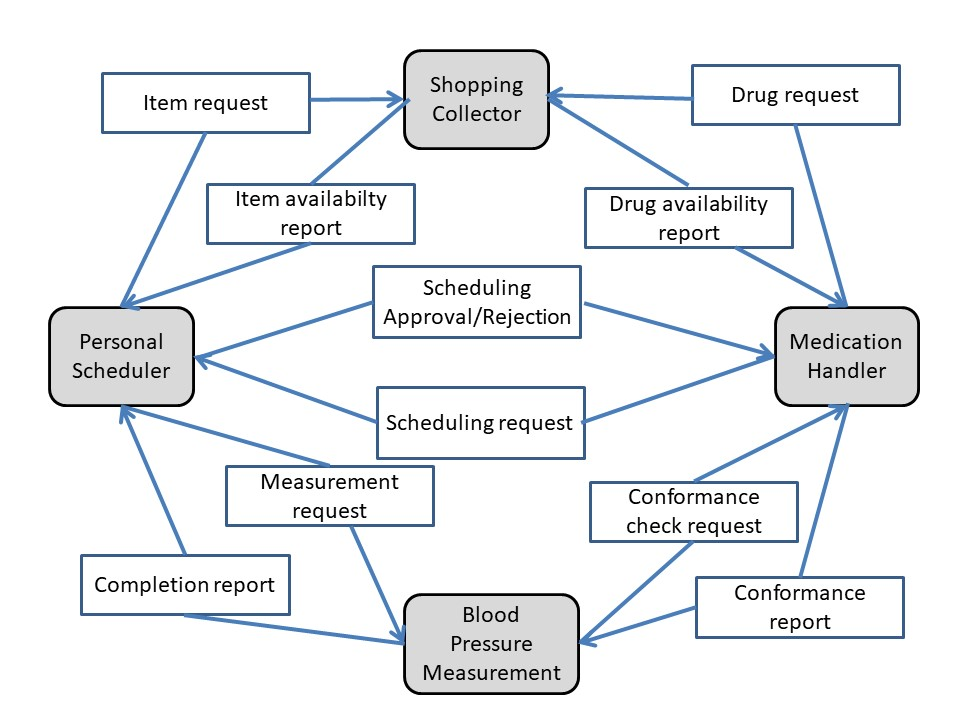
\includegraphics[width=0.6\linewidth] {Figures/Chapter5/Fog/homeCare.jpg}
	\caption[Example of home care support (SID)]{Example of home care support (SID)}
	\label{fig:homeCare}
\end{figure}


As usual Subject Behavior Diagrams (SBDs) provide a local view of the process from the perspective of individual subjects.
\\
Given these capabilities, SoS Fog designs are characterized by (i) simple communication protocols (using SIDs for a process overview) and thus, (ii) standardized behavior structures (enabled by send-receive pairs between SBDs), which (iii) scale in terms of complexity and scope.
\\
Subject-oriented Fog Computing (SFC) allows meeting ad-hoc and domain-specific requirements. As validated behavior specifications can be executed without further model transformation, stakeholders can guide the implementation of specification, representing domain-specific task flows, and make ad-hoc changes by replacing individual subject behavior specifications during runtime. Due to the distributed nature and loose coupling of subject-oriented representations, the ultimate stage of scalability could be reached through dynamic and situation-sensitive formation of edge systems.
\\
SFC structures SoS, e.g., when federating a blood pressure measurement device with a personal health scheduling systems, according to their communicating with each other. When these devices need to communicate directly with the cloud, e.g., as required in case of maintenance, or calling a specialist for medication, this link is encoded in the diagrams and executed during runtime after technical implementation. On the modeling layer the activity is a request sent to another subject, waiting until an answer is received, and processing the received answer.

\subsubsection{Execution}
Once a Subject Behavior Diagram, e.g., for the Blood Pressure Measurement subject is instantiated, it has to be decided (i) whether a human or a digital device (organizational implementation) and (ii) which actual device is assigned to the subject, acting as technical subject carrier (technical implementation) (cf. \cite{Flei12}). Typical subjects as edge devices are smart devices, which can have Internet connectivity, including smart phones, tablets, laptops, healthcare devices, etc. The subject-oriented runtime engine \cite{article:StakeHolderCentered} is then a Fog Computing infrastructure providing low-latency virtualized services and is linked with the Cloud Computing infrastructure by the same subject interaction mechanism. As there can be a variety of edge devices, such a Fog Computing platform also needs to manage and control these devices (see also foglets described below).
\\
Size, storage capacity, processing capabilities, and latency increase as we move closer to cloud computing. The subject-oriented Fog acts as an intermediate layer between the edge devices and the cloud. Edge devices request computing, storage and communication services from the Fog according to the subject-oriented communication scheme. The Fog provides local, low latency response to these requests and forwards relevant data for computationally intensive processing, long-term analytics and persistent storage over to the cloud. Figure[Fog Computing Architecture]{Fog Computing Architecture} provides a schematic visualization of this constellation, as it can be used for implementing the sample home healthcare support system.

\begin{figure}[htbp]
	\centering
	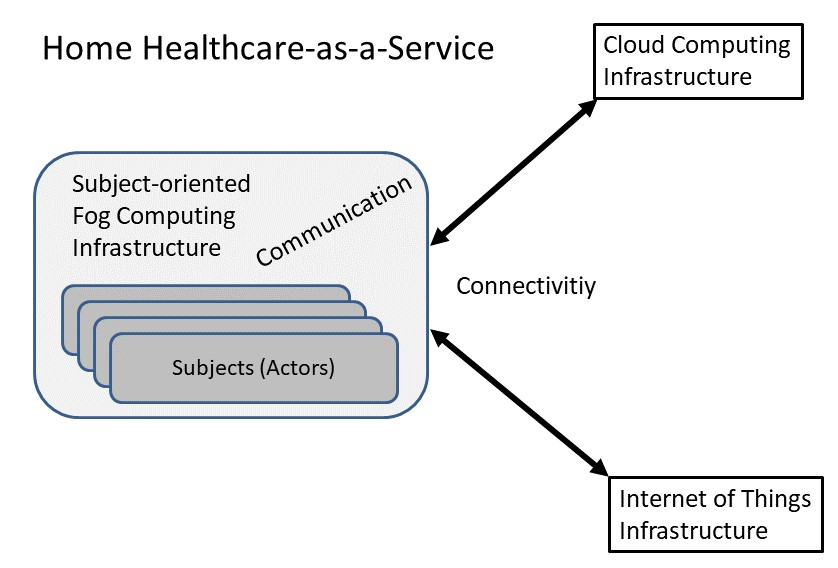
\includegraphics[width=0.6\linewidth] {Figures/Chapter5/Fog/FogArch.jpg}
	\caption[Fog Computing Architecture]{Fog Computing Architecture}
	\label{fig:FogArch}
\end{figure}

With respect to the home-healthcare example, a typical infrastructure comprises local devices and their interconnected services, such as linking the Blood Pressure Measurement to the Personal Scheduler. These subjects can be either linked to an IoT SoS, e.g., coupling several sensor systems, or to Cloud services, as for accessing public databases when checking reference or availability data, depending on the state of affairs in the home healthcare setting.
\\
Fog nodes are subject carriers representing resources including hardware (computing, networking and storage) capabilities. They provide ‘local’ real-time data processing capabilities, and, despite multi-tenancy, can execute applications in isolation to prevent unwanted interference from other processes. Policies to control service orchestration, filtering, and for adding security can be implemented dedicating a specific control subject, since the primary scheme of control is choreography.
\\
The approach scales, due to the decentralized management mechanisms allowing to setup, and configure a large number of devices in the Fog. In this context, subjects correspond to foglets (cf. \cite{article:OoTAnalytics}), i.e. software agents for each fog node, monitoring the state of the node and services. A subject can use abstraction tier APIs to monitor the state associated with (physical) devices and services deployed on this device. It analyses the entire information (encoded in an SBD), and delivers it to receivers linked through messages for further processing. These subjects can also perform lifecycle activities. As demanded by Vaquero et al. \cite{article:FiningwayFog}, SFC comprising a fog abstraction layer provides uniform programmable interfaces for resource control and management.
\\
According to the S-BPM concepts, normalization can be used to abstract essential behavior patterns. For instance, in case Blood Pressure Management requires a machine-dependent procedure, its action behavior (performing functions) as a subject can in principle contain many internal functions which are performed in sequence, in order to accomplish an assigned task. In these sequences of internal functions, no sending and receiving nodes are included. Accordingly, extensive and therefore confusing behavior diagrams can be avoided. Since these sequences of internal functions are not important for communication, model representations can be simplified, and normalized behavior can lead to larger functions by hiding functional details. Actually, for the sake of understanding the home healthcare setting, the subjects shown in Figure \ref{fig:homeCare} have been normalized.
\\
In case the communication patterns are generalized, the process-network feature of S-BPM facilitates representation. For instance, when the Shopping Collector needs to collect sensor data from various storage devices, such as a refrigerator or a food isle, its communication requests and the respective replies can be denoted in a summative way. In SFC this feature helps representing mutually dependent processes, i.e., when subjects of a near-edge process communicate with subjects of other (near-edge) processes. As shown in Figure 5 the Home care near-edge process interacts with the Goods delivery process through the Personal Scheduler. In this case, the interaction is not further detailed, rather indicated through directed links. The same holds for the interaction between the Shopping Collector and the Medication Handler, which helps ensuring the quality of drug support in the Medicare process.

\begin{figure}[htbp]
	\centering
	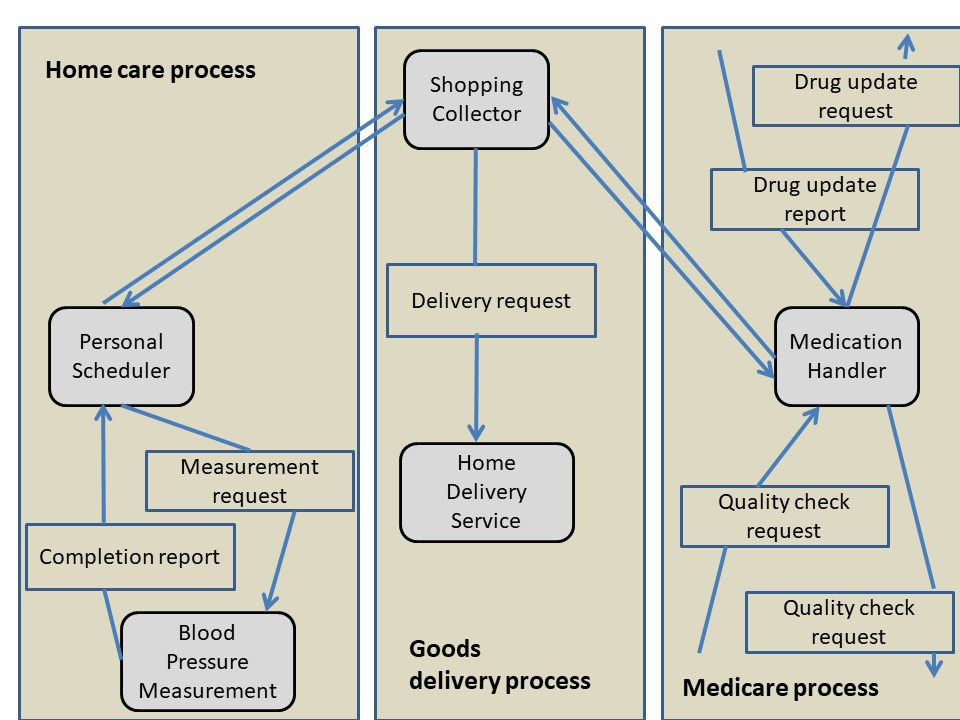
\includegraphics[width=0.6\linewidth] {Figures/Chapter5/Fog/InteractionHomeCare.jpg}
	\caption[Extended subject interaction diagram for the process ‘home care’]{Extended subject interaction diagram for the process 'home care'}
	\label{fig:InteractionHomeCare}
\end{figure}


For SFC implementation the open source engine UeberFlow \cite{DynamicPerspective} can be used. Hereby, SFC actions or tasks are ordered in the sequence as defined through SBDs and SIDs. The Workflow Specification of UeberFlow represents an entirely executable model of an application, given the subject actions and communication with others. It acts as container for so-called WorkflowUnits that are created for each subject, and captures all activities (WorkflowSteps). In addition, WorkflowUnit manages the data processed by the WorkflowSteps and its WorkflowFunctions. Consequently, Fog applications are executed through WorkflowSteps.
\\
Thereby, the WorkflowFunctions are the most fine-grained units of execution in the UeberFlow Language meta-model, and define the actual execution logic of a WorkflowStep, its prerequisites and results. Once a step is triggered, a specific sequence of WorkflowFunctions is executed. The WorkflowFunctions can be one of 6 different types. For each of them an Actor has been implemented utilizing the Akka framework (http://akka.io/). Hence, an instance in UeberFlow is equivalent to all actor instances created in the context of this particular workflow instance. All of those actor instances are aggregated using the actor structuring and supervision mechanisms by defining a root actor representing the entire instance.

\subsection{Conclusion}
Fog Computing (FC) as a near-the-edge-computing paradigm has the potential to improve user support. When defined as a collection of various small distributed clouds deployed closer to the systems or devices at the edge of a communication network subject-oriented applications support
\begin{list}{-}{spacing}
\item wide and dense geo-distribution due to their behavior abstraction, as e.g., required for home healthcare support systems, linking not only (medical) devices at home, but also medical infrastructure (physician, pharmacy, nursing services etc.) from the region
\item low or predictable latency due to the runtime concept of parallel processing
\item cloud interplay of Fog nodes, due to separating specification from technical implementation which allows for processing data at different time scales, e.g., when monitoring body condition and supporting a patient treatment planning procedure
\item multi-agencies choreography, loosening the need for orchestration, due to the inherent concept of choreography in subject-oriented architecting. Hence, Fog actors or subjects only need to be synchronized as tight as required, e.g., when a running monitor subject requires coordination with healthcare policy implementation at the same time
\item consistency, due to mapping all respective requirements to corresponding interaction patterns. Hence, demands and capabilities can be adjusted specifying message exchange patterns, in order to ensure overall consistent system states, either through subjects working in parallel, or through information distribution triggering further subject behavior.
\end{list}
Our future standardization effort will focus on including for networking information into the subject-oriented behavior abstractions, to enable modeling stakholder-specific settings according to their case-specific needs and available Fog actors. Once stakeholders are able to edit and validate the subject behavior models, they also can deal with organizational and technical implementation details, allowing them to adapt an entire application as System-of-System dynamically. Adaptation to new policies can be implemented in this way (cf. \cite{article:SecurityMgmt}), leading to more situation-sensitive Fog applications (cf. \cite{article:FogSimToolKit}).
